\section{Experiments}\label{experiments}

In the following section we first describe the dataset and discuss interesting features of the problem. Next, we perform empirical evaluations of the proposed model across two large retail environment by showing that it can more accurately recover test data better than more elementary baselines.  We explore the model by discussing the estimation of region weights, and show that it is robust to previously unseen states. Finally, we do a preliminary inquiry into effective methods for  optimization.


\subsection{Dataset Decription}

\begin{table}[h]
    \centering
    \begin{tabular}{|c|c|c|c|}
         Store Id & Regions & Products & Time Horizon \\
         \hline
         \#1 & 17 & 15 & 8/2018 - 8/2019 \\
         \#2 & 12 & 15 & 8/2018 - 8/2019  \\
         \hline
    \end{tabular}
    \caption{Dataset Summary}
    \label{data}
\end{table}


\textbf{Stores}: We collect data from two large supermarket and retail stores in Salt Lake City, UT, USA. Each store primarily sells groceries, common household goods and clothing. Our dataset is comprised of transactions from August 2018 to August 2019.  \\
\textbf{Products}: We observe quantities sold for a set of 15 products, as well as each product's average price over the year. All of the products in our dataset are popular beverage products.

\textbf{Regions:} The data provides daily counts of quantities at the region-product level. Additionally, the locations of the products are varied in product "displays". These displays are small groups of products intended to catch the eye of the shopper. See Figure \ref{intro-fig} for an example of a product display layout. Store 1 is comprised 17 regions, and store 2 has 12. Each region represents a section of the store. In general regions tend to be constructed based the functionally of each space (e.g., pharmacy, deli, etc.). We construct a spatial graph of these regions.



\begin{figure}
    \centering
    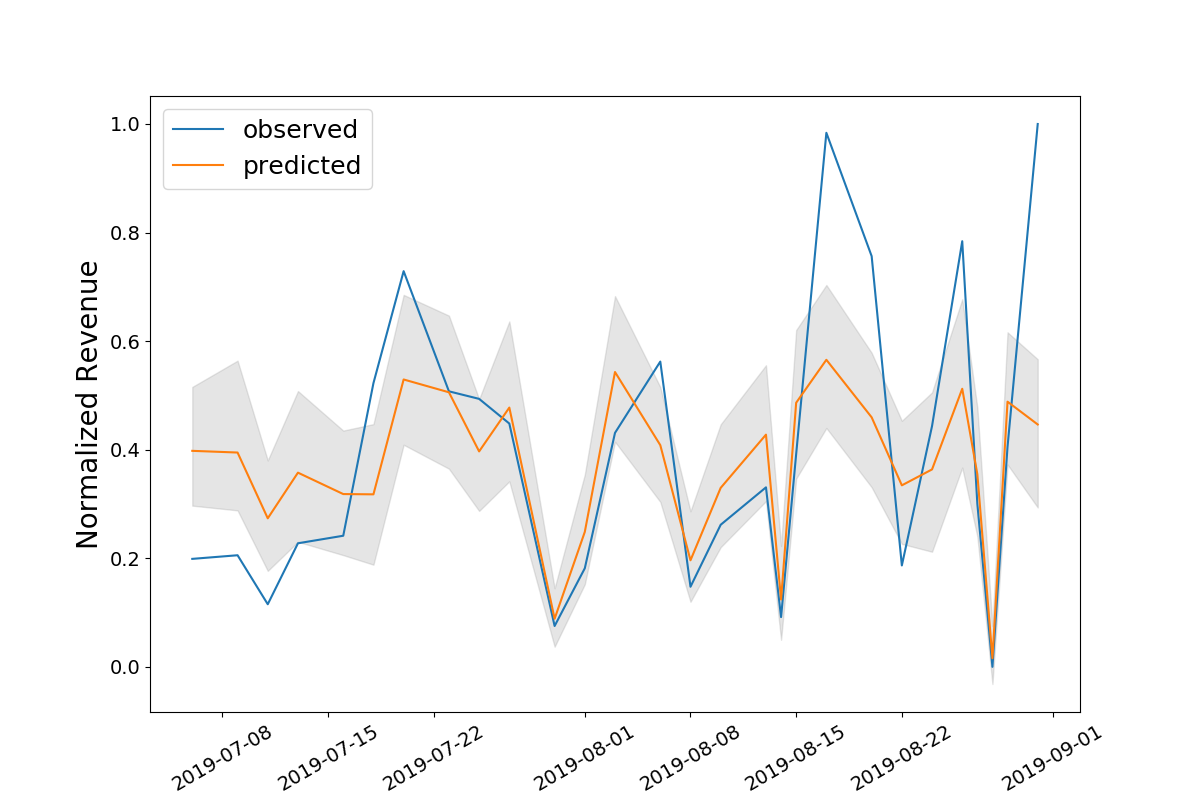
\includegraphics[scale=.3]{figs/total-ppc-hierarchical-store-2-train.png}
    \caption{Predictions and observed revenue during the test period. Revenue is aggregated to the store-level. We display the results from store 2 above. We show the posterior distribution for revenue by plotting the mean (blue line) and inner 95\% credible interval (gray shaded area). In general, the predicted revenue mirrors the behavior of the ground truth data. the proposed model correctly predicts directional changes (i.e., positive or negative) 82\% of the time.}
\label{data-overview}
\end{figure}



\subsection{Model Evaluation}

We first evaluate the effectiveness of the proposed model in predicting revenue on a test dataset. Specifically, we partition the time series into a training period from August 1, 2018 - July 4, 2019 , and a test period of July 5, 2019 to August 31, 2019. We compare the proposed model to a variety of discriminitive baselines, and simpler variants of the proposed model. We evaluate all models in terms of the following error metrics:
\begin{equation}
    \text{MSE} =  \frac{1}{nkT} \sum_{t=1}^T\sum_{i=1}^n \sum_{j=1}^k (\rho^{(t)}_{ij} - \hat{\rho}^{(t)}_{ij})^2
\end{equation}

\begin{equation}
    \text{MAE} =  \frac{1}{nkT} \sum_{t=1}^T\sum_{i=1}^n \sum_{i=j}^k | \rho^{(t)}_{ij} - \hat{\rho}^{(t)}_{ij} |
\end{equation}

where the predicted revenue is equal to the quantity times price for the $i^{th}$ product, in the $j^{th}$ region, at time, $t$: $\hat{\rho}^{(t)}_{ij} = \hat{q}^{(t)}_{ij}p_j$. To compare to the discriminitive models, we obtain a point estimate for $\hat{q}^{(t)}_{ij}$ by computing the mean of the samples taken from posterior predictive distribution.




\begin{table}
        \centering
        \caption{Evaluation of the proposed model}
        \label{ppc-results}
        \begin{tabular}{c|c|c|c|c|}
             \cline{2-5}
              & \multicolumn{2}{c}{Store 1} & \multicolumn{2}{c|}{Store 2} \\
              Environment Model & MSE & MAE & MSE & MAE \\
            \hline
             OLS  & 2845.61 & 28.01 & 4816.41  & 34.81 \\
             RF  & 2908.73 & \textbf{26.77} & 5090.11  & 36.34 \\
             MLP  & 4037.91 &  34.66  & 7322.86  & 44.37 \\
             \hline
             Proposed  & \textbf{2615.32} & 27.67 & \textbf{4492.52}  & \textbf{34.48} \\
        \hline
        \end{tabular}
\end{table}


\subsubsection{Baseline Approaches}
The proposed model is a generative environment model and is able to draw samples from the full posterior distribution of revenue, $\rho^{(t)}$.  We also compare to the following discriminative prediction models:
\begin{itemize}
    \item \textbf{Linear Regression (OLS)}: Classical least squares regression that decomposes predicted quantity as a linear function of weights: $\hat{q}^{(t)}_{ij} = \textbf{X} \textbf{w} + b$.
    \item \textbf{Random Forest (RF)}: An ensemble regressor that learns many decisions trees and averages over the labels in each terminal node to compute, $\hat{q}^{(t)}_{ij}$. We use 100 trees.
    \item \textbf{Multilayer Perceptron (MLP)}: A simple neural network with two hidden layers of dimensions 256, and 128 with ReLU activations, MSE loss, and stochastic gradient descent optimizer.
\end{itemize}

We use the same features for all baselines. The features used in the experiment are described above.

\subsubsection{Results}

We report the results in Table \ref{ppc-results}. Additionally, predictions over the test set are plotted in Figure \ref{data-overview}. Overall we have the following observations from the experiment.

First, the proposed model is overall more accurate at predicting future states than baselines.  In particular, the proposed model yields the smallest MSE scores. MSE give a higher penalty to large errors, so in general the proposed model tends to make fewer, bad mistakes than all other baselines. This result holds both in store 1, and store 2. Additionally the proposed model minimizes the MAE score in store 2, but  is beat out by only the Random Forest baseline for store 1. Upon closer analysis we see that the Random Forest baseline has the second largest MSE score in store 1, which indicates that the Random Forest regressor has a higher variance than the proposed model. Overall, the proposed model is better or comparable to all baselines in both retail stores.

Second, the use of prior information in the proposed model allows it to perform better than the discriminitive baselines. Because the proposed model is a generative, Bayesian regression model we are able to set key hyperparameters at values according to our prior knowledge. For example, we know that retail sales increase on the weekends. By guiding the estimation of model parameters through the use of human knowledge the proposed is able to achieve prediction performance superior to OLS, RF, and the MLP in nearly all cases.

\begin{figure*}[t!]
\centering
\subfloat[Store 1]{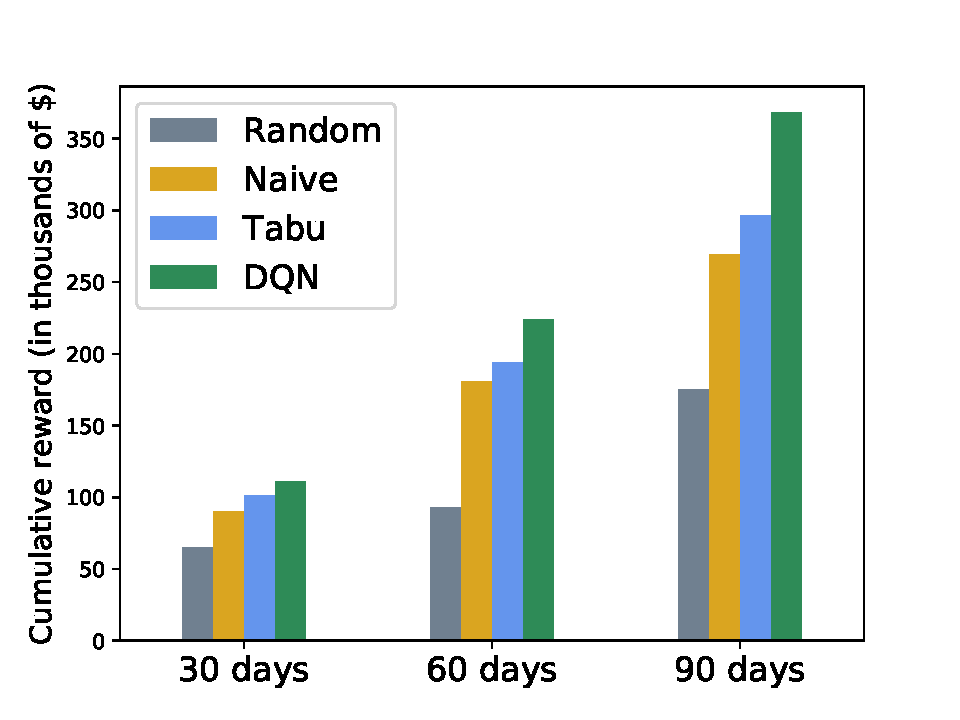
\includegraphics[width=0.45\linewidth]{figs/optimization-store-1.pdf}}
\subfloat[Store 2]{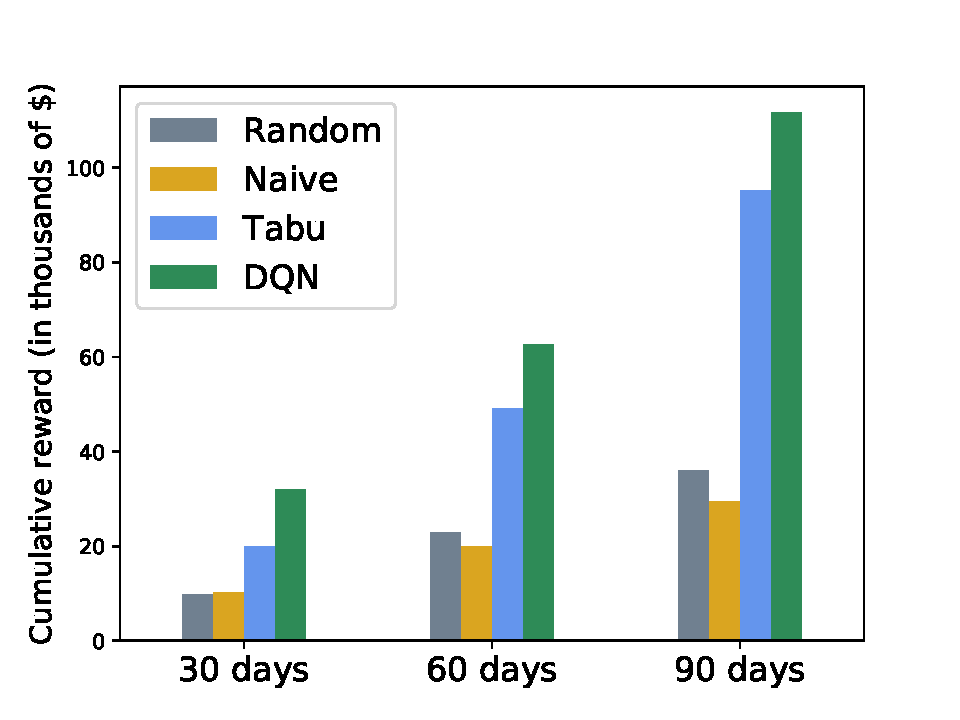
\includegraphics[width=0.45\linewidth]{figs/optimization-store-2.pdf}}

\vspace{-4mm}
\caption{A comparison of three search algorithms across store 1 and store 2. We vary the episode length in 30 day increments (i.e., 30, 60, and 90 days in the future). The DQN algorithm is superior in all cases. Additionally, we observe that as the episode length increases so does the relative effectiveness of the DQN. The DQN agent excels in the longer episode settings because it is able to learn important, longer term strategies. On average, DQN offers an improvement of 24.5\% over Tabu search in terms of cumulative test reward.}
\label{optim}
\vspace{-4mm}
\end{figure*}


\subsection{Optimization Techniques}



In this section we perform a preliminary study into various search algorithms to solve the optimal product allocation problem with the the proposed model environment model. Because exploration and experimentation in the physical world is costly, it is often preferable to design an agent that can learn a policy offline before deploying into the online environment \cite{kaiser}. 



\subsubsection{Search Algorithms}
To this end we compare four methods to search the problem  space: random search, naive search, Tabu search, and Deep Q-Learning
\begin{itemize}
    \item \textbf{Random Search} A search algorithm that relies on a totally random policy: at each time step, $t$ choose a random action.
    \item \textbf{Naive Search} The naive strategy in this case is simply ``do nothing." At each time step, we do not move any products and do not deviate from the initialized allocation policy. This baseline allows us to assess whether searching and exploration is useful at all.
    \item \textbf{Tabu Search}: A local neighborhood search algorithm that maintains a memory structure called a ``Tabu'' list. The ``Tabu'' list is comprised of recent actions to encourage exploration and avoid getting trapped in local maxima. We implement the Tabu algorithm with a ``Tabu'' list of the previous 50 actions. We treat the local neighborhood search as the enumeration over set of feasible actions given the current state, $s_t$.
    \item \textbf{Deep Q-Learning (DQN)}: A reinforcement learning algorithm that utilizes a neural network to approximate the state-action function, $Q(s, a)$. The DQN typically employs an $\epsilon\text{-greedy}$  strategy for exploration. The exploration probability, $\epsilon$ is typically annealed throughout training. DQN has been shown to be effective for learning policies in complex, dynamic environments such as Atari \cite{mnih}, Go \cite{silver-16} \cite{silver-17}, and ride dispatching \cite{lin-msu}, and traffic signal control \cite{intellilight}. We train our DQN using 50,000 training iterations prior to the test period.
\end{itemize}

\subsubsection{Policy Evaluation}



In this section we conduct a policy evaluation experiment. We randomly fix the initial environment state and allow each of the search algorithms listed above to interact with the environment according to its corresponding strategy in a test period of one episode. The state in store 1 is initialized with 96 product-region pairs, while the state in store 2 has 30. We record the total reward accumulated by each agent during the entire episode. For each store, we vary the episode length in 30 day increments: 30, 60, and 90 days in the future. This allows us to evaluate whether longer rollouts have an effect on the policy of each agent. The results of the policy evaluation experiment are reported in table \ref{optim}.

In general, we see that DQN is the most effective search algorithm in both stores, and across all three episode settings. In each case, it accumulates the most total reward in the test episode. On average, DQN is 24.5\% better than Tabu, in terms of cumulative test reward. Tabu is the second most effective search strategy, beating out the random and naive search heuristics in all cases. Interestingly, the naive search baseline of ``do nothing'' is more effective than random searching in store 1, but not in store 2. 

Additionally, it appears that as the episode length is increases, so too does the relative effectiveness of DQN as compared to Tabu. In the store 1, 30 day episode setting, DQN exceeds Tabu by \$10k. This difference increases to \$30k for 60 days and \$72k for 90 days. In store 2 we see a similar effect. The difference between DQN and Tabu increases from \$12k to \$13.5k to \$16k in the 30, 60, and 90 day settings respectively. Not only is DQN more effective, but its performance relative to other baselines gets better with longer episodes. 

DQN excels as episode length increases in large part because the underlying $Q$-function is an approximation of discounted, expected reward over time. This allows the agent to potentially think multiple steps ahead and take a set of actions that yield low immediate reward, but higher reward in later steps. Conversely, the random and Tabu search baselines are short-term or greedy search algorithms. Especially in the case of Tabu; at each time step, an action is solely selected based on what will maximize short-term reward. These results suggest that the correlations between spatial allocation and sales is complex and dynamic. Thus both of the two baselines achieve sub-optimal policies.

It is also interesting to note the behavior of the naive search compared to the random strategies across the two stores. In store 1, the environment is initialized with an allocation strategy that already has many product placements (96). We see that the naive strategy is a strong baseline, and is superior to the random policy in each of the 30, 60 and 90 day settings. However, in store 2 where the initial allocation is more sparse (30 placements), the random policy is better than or equal to the naive search. This suggest that as more products are placed it is more difficult to find incremental improvements in the allocation strategy. 


